%
% -- Manlio Modugno

\documentclass{beamer} 
\usepackage{eulervm}
%\usepackage{booktabs}
\usepackage{listings}
\usepackage{bold-extra}
\usepackage{cancel}
\usepackage{fancybox}
\usepackage{soul}
\usepackage[english]{babel}
\usepackage[utf8]{inputenc}
\usepackage{hyperref}
\usepackage{amsmath}
%\hypersetup{colorlinks=true,urlcolor=blue}

\newcommand{\codefont}{\fontsize{6}{8}\selectfont}
\lstset{language=[Sharp]C, 
captionpos=b, 
frame=lines,
lineskip= 1pt, %space between lines
basicstyle=\codefont, 
keywordstyle=\color{blue}, 
commentstyle=\color{green}, 
stringstyle=\color{red}, 
numbers=left, 
numberstyle=\tiny, 
stepnumber=2,
numbersep=5pt,
breaklines=true, 
breakatwhitespace=false,
showstringspaces=false,
frame=single,
tabsize=2,
emph={double,bool,int,unsigned,char,true,false,void},
emphstyle=\color{blue},
emph={Assert,Test},
emphstyle=\color{red},
emph={[2]\using,\#define,\#ifdef,\#endif},
emphstyle={[2]\color{blue}}
}


\mode<presentation>
\definecolor{title_color}{RGB}{2,128,181} 
\usetheme{Ilmenau}
\usecolortheme[named=title_color]{structure}
\setbeamercolor{palette quaternary}{use=structure,fg=black,bg=white} %header footer color
\useoutertheme[subsection=false]{smoothbars}
\setbeamercovered{transparent}
\setbeamertemplate{navigation symbols}{}
\setbeamerfont{subsection in toc}{size=\scriptsize}

\title{Larman - OOA/D}
\author{Manlio Modugno}
\institute[GMTechnologies] 

\date[]{OOAD}

\subject{}

\graphicspath{{img/}}
\pgfdeclareimage[height=0.6cm]{mfg-logo}{img/mfgLogo}
\logo{\pgfuseimage{mfg-logo}}

%
% Content start
%
\begin{document}
\begin{frame}
  \titlepage
\end{frame}

\begin{frame}
  \frametitle{Topics}
  \tableofcontents
\end{frame}


\section{Intro}
\subsection{Intro}
\begin{frame}
  \frametitle{Intro}
  \begin{itemize}
	\item<+-> ``owning a hammer doesn't make one an architect''..
	\item<+-> i.e. knowing a programming language doesn't imply to be an OO programmer..
	\item<+-> UML id different from ``thinking in objects''... UML is a (visual) tool...
	\item<+-> Assign responsibility, spot collaboration.. are critical in OOA/D
   \end{itemize}
\end{frame}

\section{Most Important Learning Goal}
\subsection{Most Important Learning Goal}
\begin{frame}
  \frametitle{Most Important Learning Goal}
  \begin{itemize}
	\item<+-> \textbf{A critical ability in OO development is to skillfully assign responsibilities to software objects}
	\item<+-> We'll see 9 fundamental principles ... GRASP patterns
   \end{itemize}
\end{frame}

%\section{What is Analysis and Design?}
\subsection{What is Analysis and Design?}
\begin{frame}
	\frametitle{Layering}
  	\begin{itemize}
	\item<+-> Analysis is an investigation of the problem and requirements...
	\item<+-> Design is a (conceptual) solution that fulfills the requirements.. 
	\item<+-> ``..do the right thing (analysis), and do the thing right (design)..''
	\item<+-> In OO analysis find and describe concepts in the domain problem (e.g. Flight, Plane, etc)
	\item<+-> In OO design define software objects and how they collaborate to fulfill requirements
	\item<+-> Remember OODesign = OOProgramming !
   \end{itemize}
\end{frame}

\section{Example}
\subsection{Example}
\begin{frame}
	\frametitle{Example: Dice game, define use cases}
	\begin{itemize}
	\item<+-> \textbf{Define Use Cases:} write stories/scenarios of how people use application
	\item<+-> \textbf{Play a Dice Game:}  Player requests to roll the dice. System presents results: If the dice face value totals seven, player wins; otherwise, player loses 
   \end{itemize}
\end{frame}

\begin{frame}
	\frametitle{Example: Dice game, define a domain model}
	\begin{itemize}
	\item<+-> OOA creates a description of the domain from the perspective of objects..
	\item<+-> ..identifies concepts, attributes and associations that are noteworthy
   \end{itemize}
\end{frame}

\begin{frame}
	\frametitle{Example: Dice game, define a domain model}
	A domain model is not a description of software objects! It's a visualization of real-world domain
	\begin{center}
	\fbox{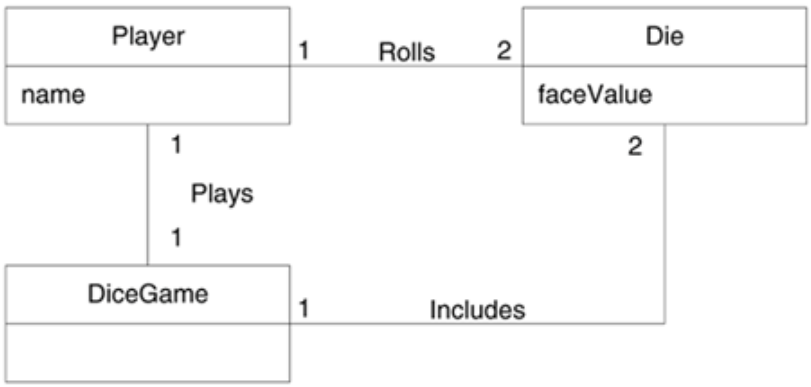
\includegraphics[scale=0.2]{domainModel}}
	\end{center}
\end{frame}

\begin{frame}
	\frametitle{Example: Dice game, assign object responsibilities, draw interaction diagram}
	OO Design defines software objects and their responsibilities and collaborations. Keep in mind the 
	difference between real world and software one.. ``Software object designs and programs do take some inspiration from real-world domains, but they are not direct models or simulations of the real world''
	\begin{center}
	\fbox{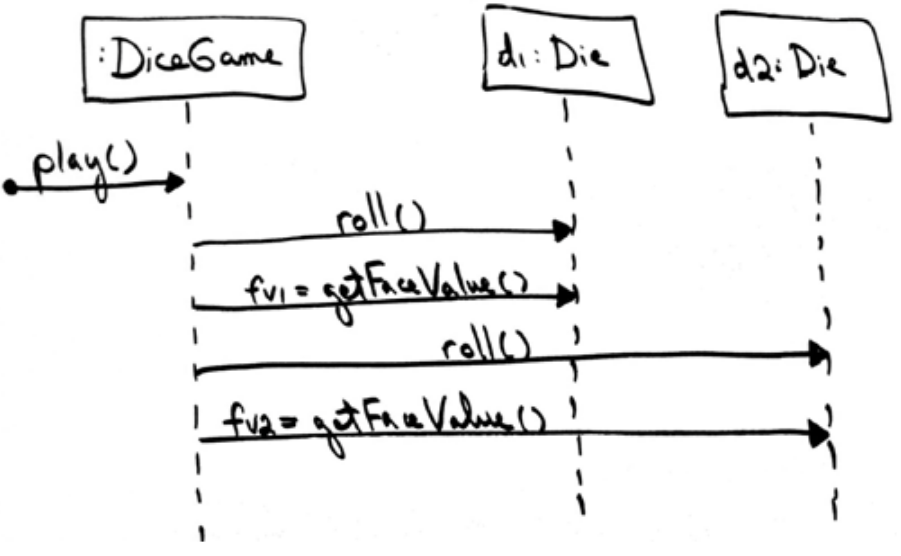
\includegraphics[scale=0.2]{interaction}}
	\end{center}
\end{frame}

\begin{frame}
	\frametitle{Example: Dice game, define design class diagrams}
In addition to the dynamic view, a static one can be created.. this is different from the diagram depicted in domain model phase..but also similar..lower representational gap
	\begin{center}
	\fbox{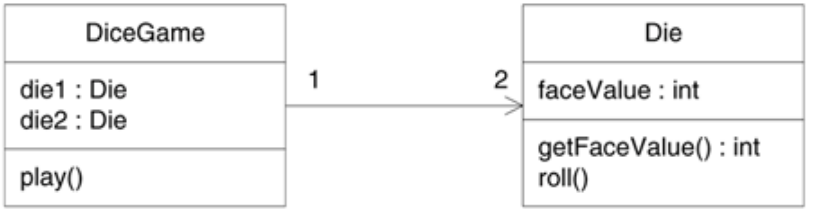
\includegraphics[scale=0.2]{classDiagram}}
	\end{center}
\end{frame}

\section{What is UML?}
\subsection{What is UML?}
\begin{frame}
	\frametitle{What is UML?}
	\begin{itemize}
		\item<+-> \textbf{def.} is a visual language for specifying, constructing and documenting the artifacts of systems
    \end{itemize}
\end{frame}


\subsection{Three Ways to Apply UML}
\begin{frame}
	\frametitle{Three Ways to Apply UML}
	\begin{itemize}
		\item<+-> \textbf{UML as sketch:} informal diagrams to \underline{explore} problems / existing solutions
		\item<+-> \textbf{UML as blueprint:} detailed diagrams for reverse / forward engineering
		\item<+-> \textbf{UML as programming language:} complete executable specification
		\item<+-> ...we use \textit{UML as sketch}
    \end{itemize}
\end{frame}

\begin{frame}
	\frametitle{"Silver Bullet" Thinking}
	\begin{itemize}
    \item<+-> ``There is no special tool or technique in software that will make a dramatic order-of-magnitude difference in productivity, defect reduction, reliability, or simplicity.''
    \item<+->  ``Tools don't compensate design ignorance''
    \item<+-> A person not having good OO design and programming skills who draws UML is just drawing bad designs
    \end{itemize}
\end{frame}

\subsection{Three Perspectives to Apply UML}
\begin{frame}
	\frametitle{Three Ways to Apply UML}
	The same UML diagram notation can be used for different areas..
	\begin{itemize}
		\item<+-> \textbf{Conceptual perspective:} describe things in real world or in a domain of interest 
		\item<+-> \textbf{Specification (software) perspective:} describe software abstraction/components ignoring particular language implementation
		\item<+-> \textbf{Implementation (software) perspective:} describe software implementation using a program language
    \end{itemize}
\end{frame}

\end{document}
